\documentclass[a4paper]{article}

%% Language and font encodings
\usepackage{polski}
\usepackage[polish]{babel}
\usepackage[utf8x]{inputenc}
\usepackage[T1]{fontenc}
\usepackage{pdfpages}
\usepackage{indentfirst}
\usepackage{listings}
\usepackage{isotope}

\usepackage{csvsimple}
\setlength{\tabcolsep}{2pt}

% Adjust penalties
\brokenpenalty=1000
\clubpenalty=1000
\widowpenalty=1000

%% Sets page size and margins
\usepackage[a4paper]{geometry}

%% Useful packages
\usepackage{amsmath}
\usepackage{graphicx}
\usepackage[colorlinks=true, allcolors=blue]{hyperref}
\usepackage{booktabs}
\usepackage{cancel}
\usepackage{tikz}

\usepackage{float}

\renewcommand\thesection{\arabic{section}.}
\renewcommand\thesubsection{\arabic{section}.\arabic{subsection}.}
\renewcommand\thesubsubsection{\arabic{section}.\arabic{subsection}.\arabic{subsubsection}.}

% The following commands are not supported in PSTricks at present
% We define them conditionally, so when they are implemented,
% this pgf file will use them.
\ifx\du\undefined
  \newlength{\du}
\fi
\setlength{\du}{15\unitlength}

\newcommand{\Vsp}[1]{\vtop to #1 {}}
\newcommand{\Hsp}[1]{\hbox to #1 {}}
\newcommand{\Small}{\scriptsize}

\title{Sprawozdanie nr 6}
\date{}


\begin{document}

\begin{center}
\begin{tabular}{|p{5.5cm}|l|l|c|}
    \hline
	% Row 1.1  
	    Wydział \Vsp{4mm} &
	    \multicolumn{1}{|l}{Dzień} &
	    poniedziałek $17^{15} - 19^{30}$ &
	    Nr zespołu \\
	% Row 1.2
	    \mbox{\small{Matematyki i Nauk Informatycznych}} &
	    \multicolumn{1}{|l}{Data}  &
	    &
	    \multicolumn{1}{c|}{\Large{18}} \\
    
    \hline
	% Row 2.1 
	    Nazwisko i Imię: &
	    \Small Ocena z przygotowania &
	    \Small Ocena ze sprawozdania &
	    \Small Ocena Końcowa \\
	% Rows 2.2-2.4
	    1. Jasiński Bartosz & & &\\
	    2. Sadłocha Adrian & & & \\
	    3. Wódkiewicz Andrzej & & & \\

    \hline
    % Row 3.1
	    \multicolumn{2}{|l|}{Prowadzący \Vsp{4mm}} &
	    \multicolumn{2}{|l|}{Podpis prowadzącego} \\  
    % Row 3.2
    	\multicolumn{2}{|l|}{dr hab. Katarzyna Grebieszkow} &
    	\multicolumn{2}{|l|}{} \\    	
    \hline
\end{tabular}
\label{pieczatka}
\end{center}

{\let\newpage\relax\maketitle}
\setcounter{secnumdepth}{2}


\section{Opis ćwiczenia}
Ćwiczenie miało na celu zbadanie stopnia osłabienie promieniowania $\gamma$ przy przejściu przez 3 różne materiały:
\begin{enumerate}
	\item{Ołów - Pb}
	\item{Miedź - Cu}
	\item{Aluminium - Al}
\end{enumerate}


\subsection{Wstęp teoretyczny}
\textbf{Promieniowanie $\gamma$} jest to obok promieniowania $\alpha$ oraz $\beta$ jedno z trzech podstawowych rodzajów promieniowania występujących w przyrodzie. Jest ono wysokoenergetyczną formą promieniowania elektromagnetycznego, o energii kwantu większej od 50 keV. Podczas zachodzenia przemiany $\gamma$ następuje pozbycie się nadmiaru energii z jądra atomowego. Liczba nukleonów w jądrze pozostaje bez zmiany. Pozostałe rodzaje promieniowania polegają na emitowaniu cząstek. Odpowiednio dla przemiany $\alpha$ jest to cząstka która składa się z 2 protonów i 2 neutronów, czyli jest jądrem izotopu atomu helu, jest to najmniej przenikliwe promieniowanie z wymienionych. Przemiana $\beta$ dzieli się na dwa rodzaje $\beta^{-}$ oraz $\beta^{+}$, w pierwszej emitowany jest elektron oraz antynetrino elektronowe, natomiast w drugim pozyton i neutrino elektronowe. \\
Promieniowanie $\gamma$ przenika przez materiał, podczas tego procesu oddziaływuje ono z elektronami oraz jądrami atomów. Występują 3 zjawiska w których bierze udział cząstka $\gamma$:
\begin{enumerate}
	\item{rozpraszanie Komptonowskie}
	\item{zjawisko fotoelektryczne}
	\item{tworzenie par elektron-pozyton}
\end{enumerate}
 
\textbf{Zjawisko Comptona} polega na rozpraszaniu się cząstek promieniowania na elektronach które możemy traktować jako swobodne (znajdują się one na ostatnich orbitach w atomie). Jako rezultat oddziaływania otrzymujemy kwant $\gamma$ który zmiania kierunek oraz oddaje od część energii dla elektronu.\\
\textbf{Zjawisko fotoelektryczne} zachodzi pomiędzy cząstkami $\gamma$ a elektronami znajdującymi się na orbitalach blisko jądra atomowego. Po jego zajściu kwant zostanie pochłonięty i elektron zostanie oderwany od atomu oraz otrzyma pewną energię kinentyczną.\\
 \textbf{Tworzenie się par elektron-pozyton} polega na stworzeniu pary cząstek przy odziaływaniu kwantów $\gamma$ z jądrami atomowymi. Energią progową do zajścia tego zjawiska jest 1.02 MeV co jest sumaryczną energią elektronu i pozytonu.\\
W naszym doświadczeniu jako źródła promieniowania używaliśmy \isotope[60][27]{Co} którego czas połowicznego rozpadu wynosi 5 lat. Zgodnie ze wzorem 
\begin{align*}
N(t) = N_0 e^{−\lambda t}
\end{align*}
gdzie:
$N(t)$ – liczba jąder promieniotwórczych, które nie uległy rozpadowi do chwili czasu t,
$N_0$ – liczba jąder promieniotwórczych w chwili czasu t = 0, $N(0) = N_0$ , $\lambda$ – stała, zwana stałą rozpadu.\\
Promieniowanie wysyłane przez naszą próbkę podczas trwania eksperymentu możemy traktować jako stałe ponieważ czas trwania doświadczenia (~1h) jest znikomy w porównaniu do 5 lat.\\
Następujący wzór:
\begin{align*}
I = I_0 e^{− \mu  x}
\end{align*}
gdzie: $I(x)$ – natężenie wiązki po przejściu przez absorbent o grubości x, $I_0 = I(0)$ – początkowe natężenie
wiązki, $\mu$ – współczynnik osłabienia promieniowania gamma\\
opisuje związek natężenia wiązki wypromieniowanej po przejściu przez absorbent grubości x. Możemy go wyprowadzić w następujący sposób:
Do pochłaniania promieniowania $\gamma$ w materii przyczyniają się 3 wcześniej wymienione zjawiska. Możemy to zapisać zależnością
\begin{align*}
\mu = \mu_c +\mu_f +\mu_p
\end{align*}
do sumy włączają się zjawisko Comptona, fotoelektryczne oraz tworzenie się par elektron-pozyton.
Jako że zmieniejszenie się natężenia kwantów $\gamma$ jest wprost proporcjonalne do grubości meterii przez którą one przelecą możemy zapisać następującą zależość:
\begin{align*}
−dI = B I dx
\end{align*}
z czego po scałkowaniu otrzymujemy:
\begin{align*}
I ( x)=I_0 e^{−B x}
\end{align*}
co daje nam wzór na osłabienie wiązki z współczynnikiem $B = \mu$.
W naszym doświadczeniu chcemy właśnie wyznaczyć współczynnik osłabienia $\mu$ lecz nie jesteśmy tego w stanie zrobić metodą bezpośrednią (mierząc natężenie początkowe $I_0$) ponieważ do pomiarów włączają się cząstki powstałe w wyniku przemiany $\beta$. By wyznaczyć wspomniany współczynnik posłużymy się metodą najmniejszych kwadratów w następujący sposób:\\
Logarytmujemy obie strony wyznaczonego wzoru na osłabienie promieniowania otrzymując:
\begin{align*}
ln( I )=ln( I_0 )−\mu x
\end{align*}
teraz możemy dokonać podstawienia $ln(I) = y$ oraz $ln (I_0 ) =b$ i $\mu = a$ dzięki czemu otrzymujemy równanie prostej:
\begin{align*}
y = ax + b
\end{align*}
Z czego po przeprowadzeniu serii pomiarów możemy wyznaczyć wspomniany wczesniej współczynnik

%TODO WSPOMNIEĆ O KOLIMATORZE


\subsection{Układ pomiarowy} %TODO MOŻE WIĘCJE NAPISAĆ W OPISIE UKŁADU POMIAROWEGO
Do przeprowadzenia ćwiczenia posłużono się układem pomiarowym,
przedstawionym na rysunku \ref{uklad_pomiarowy}. Próbka umieszczona w domku osłonowym wysyła promieniowanie które jest formowane przy przejściu przez kolimator, daje trafia ono na absorbent o zadanej grubości. Po przejściu przez absorbent zostaje zliczony przez detektor który wysyła informację do komputera. Kolimator jest przydatny w celu uformowania wiązki, w przeciwnym razie gdyby kwanty $\gamma$ mogły lecieć w dowolnych kierunkach trafiały one by w takie części absorbenta w których pod wpływem rozpraszania (w którym następuje zmiana kąta) trafiały by do detektora i sztucznie zwiększały ilośc zliczeń, przez co mielibyśmy zaburzony współczynnik $\mu$.


\begin{figure}[h!]
\centering
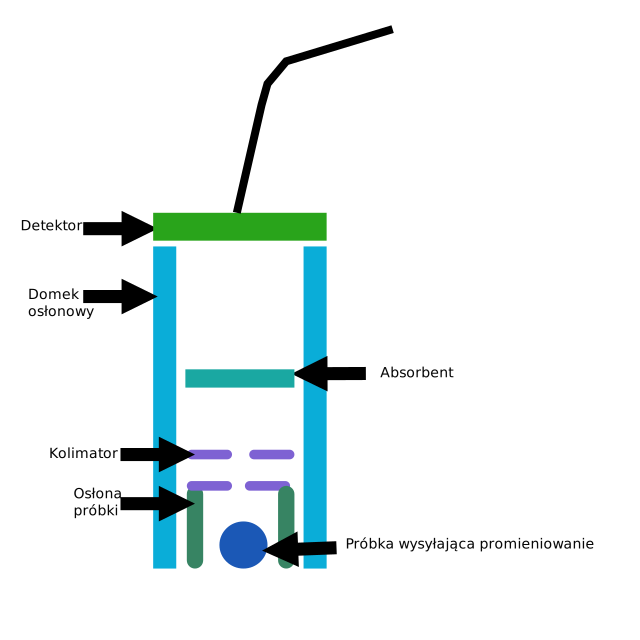
\includegraphics[scale=0.6]{schemat_ukladu}
\caption{Schemat układu pomiarowego}
\label{uklad_pomiarowy}
\end{figure}


\section{Pomiary i obliczenia}
\subsection{Pomiary grubości absorbentów}
Na początku ćwiczania otrzymaliśmy listę ze wcześniej wykonanymi pomiarami grubości absorbentów. Skorzystaliśmy z następujących wzorów w  celu wyznaczenia niepewności pomiarowych: 
\begin{align*}
S_{\bar{x}} = \sqrt{\frac{\sum_{i=1}^{10}(x_i-\bar{x})^2}{N(N-1)}}
\end{align*}
gdzie: $S_{\bar{x}}$ - niepewność typu A, $N = 10$, $\bar{x} = \frac{\sum_{i=1}^{10}x_i}{10}$. \\
Natomiast niepewność pomiaru z uwzględnieniem niepewności ekperymentatora

\begin{align*}
U_{\bar{x}} = \sqrt{S_{\bar{x}}^2 + \frac{(\Delta x)^2}{3} + \frac{(\Delta x_E)^2}{3}}
\end{align*}
dla parametrów: $\Delta x = 0.001 mm$, $\Delta x_E = 0.005 mm$

Pomiary w których występuje błąd gruby zostały przekreślone w tabelkach.

Otrzymaliśmy następujące pomiary grubości poszczególnych absorbentów:

\begin{table}[h!]

\begin{tabular}{ | l | l | l | l | l | l | l | l | l | l | l | l | l | l | l |}
\hline
 & 1 & 2 & 3 & 4 & 5 & 6 & 7 & 8 & 9 & 10 & $\bar{x}$ [mm] & $\Delta x$ [mm] & $S_{\bar{x}}$ [mm] & $U_{\bar{x}}$ [mm] \\ \hline
5 & 5.05 & 5.04 & 5.04 & 5.05 & 5.04 & 5.04 & 5.04 & 5.05 & 5.04 & 5.04 & 5.043 & 0.01 & 0.002 & 0.0018  \\ \hline
10 & 10.00 & 10.01 & 10.00 & 10.00 & 10.01 & \cancel{10.12} & 10.00 & 10.01 & 10.01 & 10.01 & 10.0056 & 0.01 & 0.002 & 0.0021 \\ \hline
15 & 14.77 & 14.78 & 14.78 & 14.77 & 14.76 & 14.75 & 14.77 & 14.78 & 14.79 & 14.78 & 14.7730 & 0.01 & 0.004 & 0.0044 \\ \hline
20 & 20.07 & 20.08 & 20.07 & 20.06 & 20.06 & 20.07 & 20.07 & 20.08 & 20.08 & 20.07 & 20.0710 & 0.01 & 0.002 & 0.0028 \\ \hline
\end{tabular}
\caption{Wyniki wielokrotnych pomiarów grubości aluminiowego absorbentu}
\label{grubosc_aluminium}
\end{table}



\begin{table}[h!]
\centering
\begin{tabular}{ | l | l | l | l | l | l | l | l | l | l | l | l | l | l | l | }
\hline
 & 1 & 2 & 3 & 4 & 5 & 6 & 7 & 8 & 9 & 10 & $\bar{x}$ [mm] & $\Delta x$ [mm] & $S_{\bar{x}}$ [mm] & $U_{\bar{x}}$ [mm] \\ \hline
2 & 1.88 & 1.89 & 1.9 & 1.88 & 1.89 & 1.9 & 1.87 & 1.89 & 1.89 & 1.88 & 1.887 & 0.01 & 0.003 & 0.0036 \\ \hline
5 & 5 & 5.01 & 5 & 5.01 & 5.01 & 5.01 & 5.02 & 5 & 5.01 & 5.03 & 5.0100 & 0.01 & 0.003 & 0.0035 \\ \hline
7 & 6.99 & 6.98 & 6.98 & 6.99 & 6.98 & 6.98 & 6.98 & 6.97 & 6.98 & 6.98 & 6.9810 & 0.01 & 0.002 & 0.0021\\ \hline
10 & 9.91 & 9.9 & 9.92 & 9.91 & 9.91 & 9.92 & 9.9 & 9.9 & 9.91 & 9.9 & 9.9080 & 0.01 & 0.002 & 0.0030 \\ \hline
12 & 11.89 & 11.9 & 11.9 & 11.89 & 11.88 & 11.89 & 11.89 & 11.9 & 11.9 & 11.89 & 11.8930 & 0.01 & 0.002 & 0.0025 \\ \hline
15 & 14.97 & 14.98 & 14.98 & 14.99 & 14.98 & 14.98 & 14.97 & 14.98 & 14.97 & \cancel{14.10} & 14.9778 & 0.01 & 0.002 & 0.0026 \\ \hline
17 & 16.99 & 16.98 & 16.98 & 16.97 & 16.99 & 16.98 & 16.98 & 16.97 & 16.98 & 16.98 & 16.9800 & 0.01 & 0.002 & 0.0025 \\ \hline
20 & 20.01 & 20.02 & 20 & 20.01 & 20.02 & 20.01 & 20.02 & 20.01 & 20.01 & 20.01 & 20.0120 & 0.01 & 0.002 & 0.0024\\ \hline

\end{tabular}
\caption{Wyniki wielokrotnych pomiarów grubości ołowianego absorbentu}
\label{pomiary_sruba}
\end{table}

\begin{table}[h!]
\centering
\begin{tabular}{ | l | l | l | l | l | l | l | l | l | l | l | l | l | l | l |}
\hline
 & 1 & 2 & 3 & 4 & 5 & 6 & 7 & 8 & 9 & 10 & $\bar{x}$ [mm] & $\Delta x$ [mm] & $S_{\bar{x}}$ [mm] & $U_{\bar{x}}$ [mm] \\ \hline
2 & 1.95 & 1.94 & 1.98 & 1.96 & 1.95 & 1.94 & 1.95 & 1.95 & 1.94 & 1.95 & 1.9510 & 0.01 & 0.004 & 0.0045\\ \hline
5 & 4.88 & 4.89 & 4.88 & 4.88 & 4.89 & 4.9 & 4.88 & 4.87 & 4.88 & 4.9 & 4.8850 & 0.01 & 0.003 & 0.0037 \\ \hline
7 & 7.07 & 7.08 & 7.08 & 7.09 & 7.09 & 7.08 & 7.09 & 7.09 & 7.08 & 7.08 & 7.0830 & 0.01 & 0.002 & 0.0025 \\ \hline
10 & 10.08 & 10.07 & 10.08 & 10.08 & 10.09 & 10.07 & 10.07 & 10.07 & 10.08 & 10.08 & 10.0770 & 0.01 & 0.002 & 0.0025\\ \hline
12 & 12.05 & 12.04 & 12.05 & 12.06 & 12.06 & 12.05 & 12.04 & 12.05 & 12.06 & 12.05 & 12.0510 & 0.01 & 0.002 & 0.0028\\ \hline
15 & 15.06 & 15.05 & 15.04 & 15.06 & 15.06 & 15.05 & 15.06 & 15.04 & 15.05 & 15.06 & 15.0530 & 0.01 & 0.003 & 0.0031\\ \hline
17 & 17.08 & 17.09 & 17.09 & 17.08 & 17.07 & 17.08 & 17.08 & 17.09 & 17.08 & 17.07 & 17.0810 & 0.01 & 0.002 & 0.0028\\ \hline
20 & 20.15 & 20.14 & 20.15 & 20.15 & 20.14 & 20.13 & 20.13 & 20.14 & 20.15 & 20.16 & 20.1440 & 0.01 & 0.003 & 0.0036\\ \hline
\end{tabular}
\caption{Wyniki wielokrotnych pomiarów grubości miedzianego absorbentu}
\label{pomiary_sruba}
\end{table}



\subsection{Promieniowanie tła}
Na początku ćwiczenia dokonaliśmy kilku pomiarów promieniowania tła (bez umieszczenia próbki promieniotwórczej w domku osłonowym) w celu zbadania średniego promieniowania które dociera do detektora z różnych źródeł np. promieniowania kosmicznego, promieniowania wysyłanego przez inne materiały. Promieniowanie tła było następnie automatycznie odejmowane od otrzymanej liczby zliczeń przez program komputerowy. Promieniowanie tła było rzędu kilkudziesięciu zliczeń w ciągu minuty.

\subsection{Badanie liczby zliczeń kwantów gamma}
Każde zliczanie kwantów gamma trafiających w detektor trwało 1 min. Dla ołowiu oraz miedzi przeprowadziliśmy 8 pomiarów (każdy z inną grubością absorbenta) oraz 4 pomiary dla aluminium.
Liczba wypromieniowanych kwantów $\gamma$ podlega rozkładowi Poissona dzięki czemu $u_N=\sqrt{N}$.\\
Niepewność $u_{\ln{N}}$ została policzona wzorem:
\begin{align*}
u_{\ln{N}} = \sqrt{(\frac{\delta \ln{N}}{\delta N})^2 u^2_N} = \sqrt{(\frac{1}{N})^2(\sqrt{N})^2} = \frac{\sqrt{N}}{N}
\end{align*}

Otrzymaliśmy następujące pomiary zliczeń w zależności od rodzaju absorbenta oraz jego grubości:\\
\begin{table}[h!]
\centering
\begin{tabular}{ | l | l | l | l | l | }
\hline
Nr & $\bar{x(u_{\bar{x}})}$ [mm] & $N(u_N)$ & $\ln{N}(u_{\ln{N}})$ \\ \hline
1 & 5.0430(0.007) & 1514(39) & 7.323(0.026)  \\ \hline
2 & 10.0056(0.007) & 1380(37) & 7.230(0.027)  \\ \hline
3 & 14.7730(0.007) & 1285(36) & 7.159(0.028) \\ \hline
4 & 20.0710(0.007) & 1226(35) & 7.112(0.029) \\ \hline
\end{tabular}
\caption{Liczba otrzymanych kwantów gamma w zależności od grubości aluminium}
\label{pomiary_sruba}
\end{table}



\begin{table}[h!]
\centering
\begin{tabular}{ | l | l | l | l | l | }
\hline
Nr & $\bar{x(u_{\bar{x}})}$ [mm] & $N(u_N)$ & $\ln{N}(u_{\ln{N}})$ \\ \hline
1 & 1.887(0.007) & 1452(38) & 7.281(0.026)  \\ \hline
2 & 5.010(0.007) & 1214(35) & 7.102(0.029)  \\ \hline
3 & 6.981(0.007) & 1048(32) & 6.955(0.031) \\ \hline
4 & 9.908(0.007) & 899(30) & 6.801(0.033) \\ \hline
5 & 11.893(0.007) & 803(28) & 6.688(0.035) \\ \hline
6 & 14.978(0.007) & 712(27) & 6.568(0.037) \\ \hline
7 & 16.980(0.007) & 565(24) & 6.337(0.042) \\ \hline
8 & 20.012(0.007) & 531(23) & 6.75(0.043) \\ \hline   
\end{tabular}
\caption{Liczba otrzymanych kwantów gamma w zależności od grubości ołowiu}
\label{pomiary_sruba}
\end{table}


\begin{table}[h!]
\centering
\begin{tabular}{ | l | l | l | l | l | }
\hline
Nr & $\bar{x(u_{\bar{x}})}$ [mm] & $N(u_N)$ & $\ln{N}(u_{\ln{N}})$ \\ \hline
1 & 1.948(0.007) & 1469(38) & 7.292(0.026)  \\ \hline
2 & 4.885(0.007) & 1346(37) & 7.205(0.027)  \\ \hline
3 & 7.083(0.007) & 1156(34) & 7.053(0.029) \\ \hline
4 & 10.077(0.007) & 1066(33) & 6.971(0.031) \\ \hline
5 & 12.051(0.007) & 961(31) & 6.868(0.032) \\ \hline
6 & 15.053(0.007) & 908(30) & 6.811(0.033) \\ \hline
7 & 17.081(0.007) & 780(28) & 6.659(0.036) \\ \hline
8 & 20.144(0.007) & 686(26) & 6.531(0.038) \\ \hline   
\end{tabular}
\caption{Liczba otrzymanych kwantów gamma w zależności od grubości miedzi}
\label{pomiary_sruba}
\end{table}

Otrzymujemy odpowiednio wykresy liniowo-liniowy oraz logarytmiczno-liniowy.
\begin{figure}[h!]
\centering
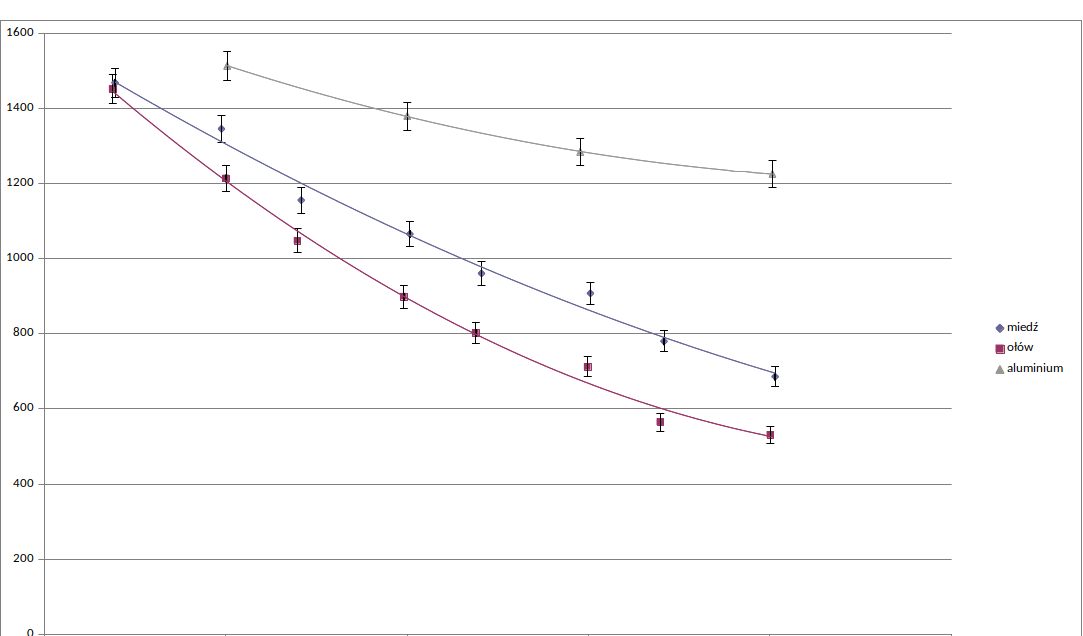
\includegraphics[scale=0.51]{liniowo_liniowy.png}
\caption{Wykres liniowo liniowy liczby zliczeń w zależności od grubości absorbentów}
\label{uklad_pomiarowy}
\end{figure}

\begin{figure}[h!]
\centering
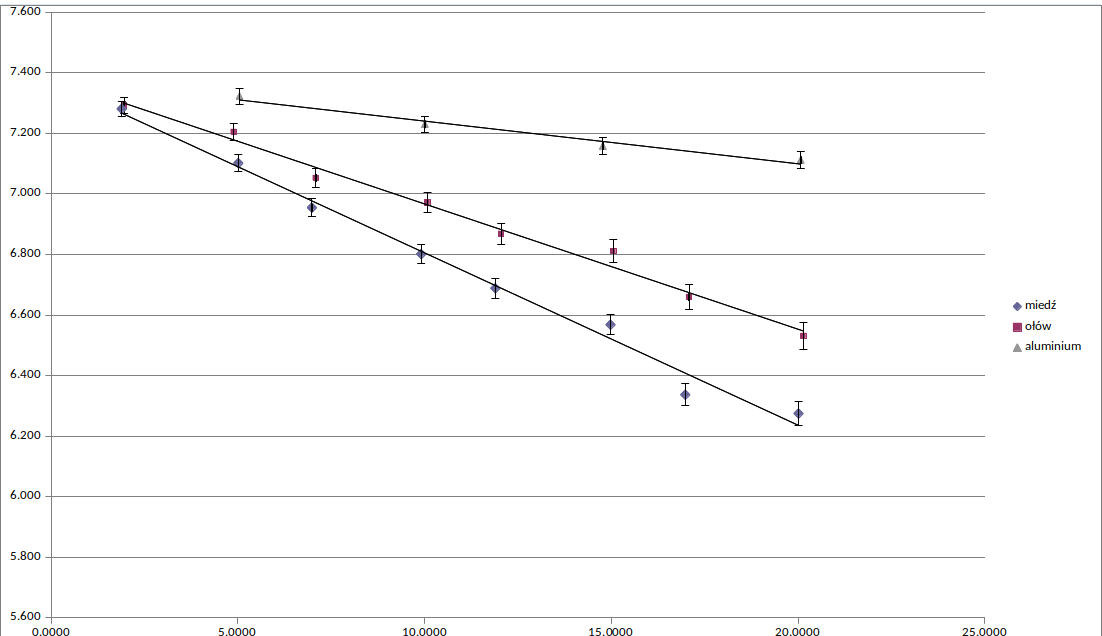
\includegraphics[scale=0.51]{ln_x_wykres.png}
\caption{Wykres logarytmiczno liniowy liczby zliczeń w zależności od grubości absorbentów}
\label{uklad_pomiarowy}
\end{figure}

\newpage
\subsection{Wyniki}
By wyznaczyć poszczególne współczynniki użyliśmy metody najmniejszych kwaratów w sposób w jaki zostało to opisane we wstępie teoretycznym. Odpowiednio otrzymujemy: \\
Aluminium:\\
$\mu_{Al} = 0.014$\\
$u_{\mu} = 0.002$\\
$b = 7.381$\\
$S_{b} = 0.022$\\
Odpowiedź: $\mu_{Al} = 0.014(0.002) \frac{1}{mm}$\\
Ołów:\\
$\mu_{Pb} = 0.056$\\
$u_{\mu} = 0.002$\\
$b = 7.374$\\
$S_{b} = 0.030$\\

Odpowiedź: $\mu_{Pb} = 0.056(0.002) \frac{1}{mm}$\\
Miedź:\\
$\mu_{Cu} = 0.041$\\
$u_{\mu} = 0.002$\\
$b = 7.381$\\
$S_{b} = 0.023$\\
Odpowiedź: $\mu_{Cu} = 0.041(0.002) \frac{1}{mm}$ \\
Co możemy porównać z wartościami tablicowymi dla poszczególnych materiałów (wyliczone przez program komputerowy)
\begin{table}[h!]
\centering
\begin{tabular}{ | l | l | l | l | l | }
\hline
materiał & MeV & $\mu$[1/mm] \\ \hline
Al & 1.33 & 0.012 \\ \hline  
Cu & 1.33 & 0.043 \\ \hline  
Pb & 1.33 & 0.062 \\ \hline  
\end{tabular}
\caption{Wartości tablicowe współczyników osłabienia promieniowania}
\label{pomiary_sruba}
\end{table}
\subsection{Wnioski}
Policzmy czy wyznaczone wartości współczynników są zgodne z wartościami talicowymi. Skorzystajmy w tym celu z testu $2\delta$ (tu dla wersji z ołowiem):
\begin{align*}
\frac{|\mu_{Pb tablicowe} - \mu_{Pb otrzymane}|}{S_{Pb}} \leq 2
\end{align*}
Jeśli powyższy test zostanie spełniony oznacza to że otrzymaliśmy poprawne współczynniki.
Mamy więc \\
\begin{table}[h!]
\centering
\begin{tabular}{ | l | l | l | }
\hline
materiał & wynik & czy zgodne \\ \hline
Al & 1.00 & TAK \\ \hline  
Cu & 1.00 & TAK \\ \hline  
Pb & 3.50 & NIE \\ \hline  
\end{tabular}
\caption{Wartości tablicowe współczyników osłabienia promieniowania}
\label{pomiary_sruba}
\end{table}\\
Z powyższego ćwiczenia możemy wyciągnąć następujące wnioski
\begin{itemize}
\item Ołów jest najlepszy absorbentem promieniowania gamma
\item Różnice pomiędzy wartościami tablicowymi a zmierzoną wartością można wytłumaczyć poprzez krótkie czasy pomiarów oraz rozkładem statsytcznym wyników które w rzadkich przypadkach mogą dawać duże rozbierzności pomiędzy wartością zbadaną a wartością tablicową
\item Wyznaczanie współczynnika osłabienia dla ołowiu charakteryzowało się największą różnicą pomiędzy wartością tablicową, a wartością zmierzoną
\end{itemize}

\end{document}
